\subsection{Classification trees}

The following section has the purpose to use tree-based classification methods to identify a model which will predict if an NBA's rookie carreer will be longer than five years.

We started to analyse the data through classification trees using the \textit{gini} minimization function. The result is a complex tree which is difficult to read.

We then decided to use cross-validation with different level of tree size to understand if it is better to take a simpler tree (without increasing the test error too much).

In figure \Fig~\ref{fig:tree_cv_plot} we can see the trend of the deviance and of the penalization factor \textit{k} for different values of tree size.

In figure \Fig~\ref{fig:tree_prune_comparison} is shown the output of the trees with different sizes.

\begin{figure}[h]
	\centering
	\begin{subfigure}{.6\textwidth}
		\centering
		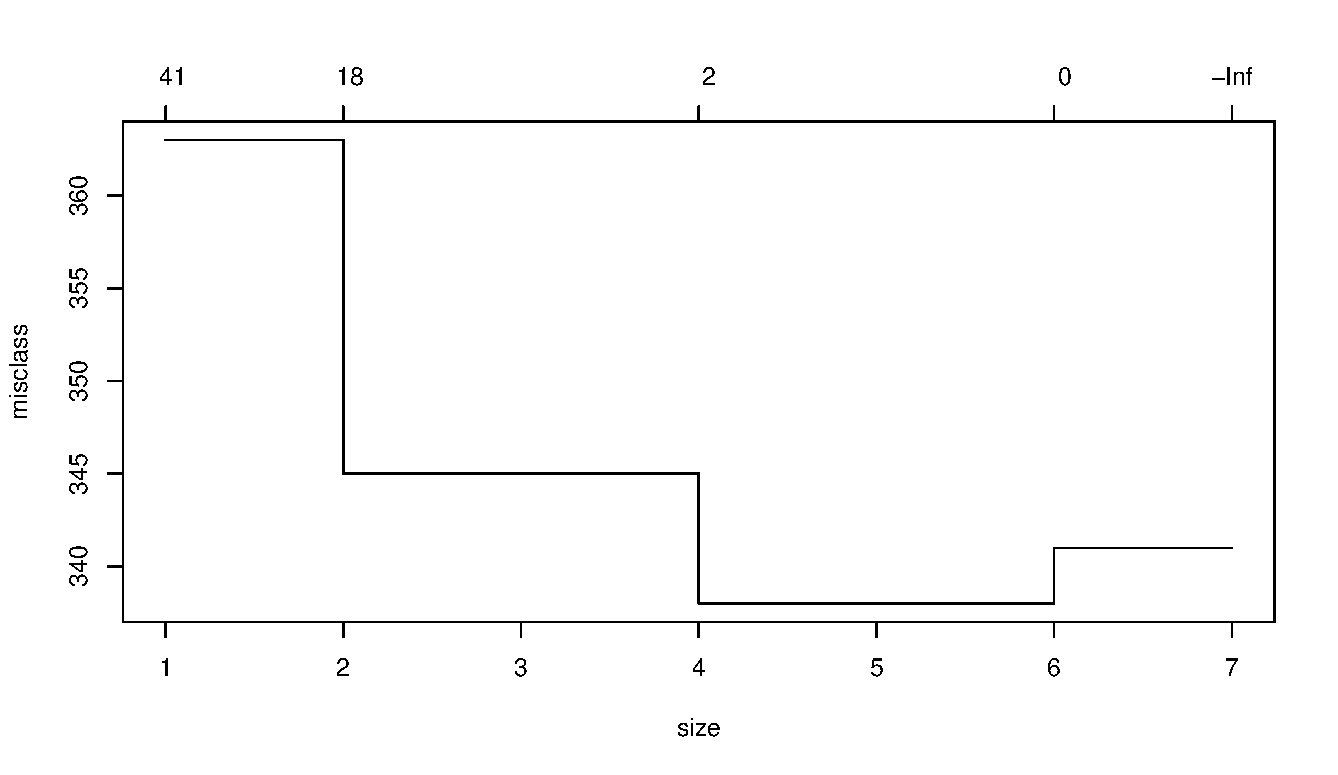
\includegraphics[width=0.5\linewidth]{ImageFiles/Classification/Trees/tree_cv_plot}
		\caption{Size (bottom), deviance (left), k (top)}
		\label{fig:tree_cv_plot}
	\end{subfigure}%
	\begin{subfigure}{.6\textwidth}
		\centering
		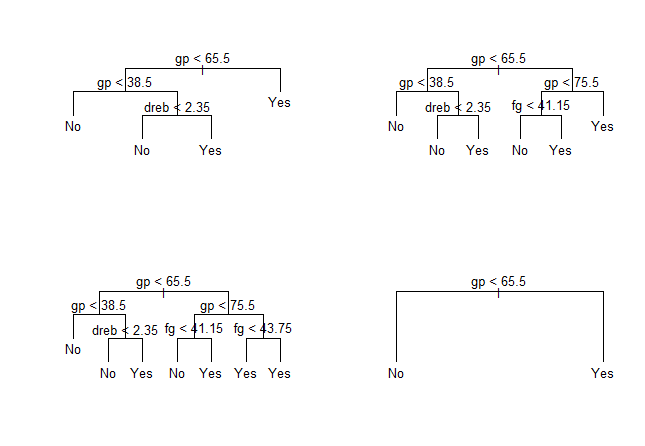
\includegraphics[width=0.5\linewidth]{ImageFiles/Classification/Trees/tree_prune_comparison}
		\caption{Different size trees}
		\label{fig:tree_prune_comparison}
	\end{subfigure}
\end{figure}

After evaluating the misclassification error rate on the train dataset and the test error rate we concluded that the best model is the one with $size = 4$.

However, all the trees do the first split on the variable \textit{gp}, meaning that this is the most important variable for the model.
